\documentclass[a4paper,12pt]{article}
\usepackage[utf8]{inputenc}
\usepackage{amssymb,amsmath,uniinput,graphicx,hyperref, multirow,siunitx}
\usepackage[section]{placeins}
\usepackage[ngerman]{babel}
\usepackage[left=3cm,right=3cm,top=3cm,bottom=3cm]{geometry}
\renewcommand{\familydefault}{\sfdefault}
\setlength{\belowcaptionskip}{6pt}
\hypersetup{pdfinfo = {
	Title={Versuchsprotokoll zu Positronen im Festkörper},
	Author={Knut Kiesel, Tobias Pook},
	Keywords={Teilchenfalle}
}}


\graphicspath{ {../pictures/} }
\title{Laborpraktikum Teilchenphysik\\ Lebensdauer von Positronen im Festkörper}
\author{Knut Kiesel\\Tobias Pook}
\date{\today}

\begin{document}
\maketitle
\vspace{5cm}
\tableofcontents
\thispagestyle{empty}
\newpage
\setcounter{page}{1}

\section{Ziel des Versuches}
Ziel des Versuches ist der Aufbau und die Inbetriebnahme einer Messstation,
die in der Lage ist die Lebensdauer von Positronen in Festkörpern in der
Größenordnung von $\si{ps}$ zu messen.

Hierzu wird $^{22}$Na verwendet, welches beim Zerfall in $^{22}$Ne
zuerst ein γ-Quant der Energie $1.28\si{MeV}$ abgibt und dann ein Positron emittiert.
Nach einer vom Festkörper abhängigen Zeit annihiliert das Positron unter Aussendung
von 2 bis 3 γ Quanten mit einer Energie von $0.511\si{keV}$.
Durch das messen der Zeitdifferenz zwischen dem ersten γ-Quant des Übergangs und dem
γ aus der Annihilation kann die Lebensdauer des Positrons bestimmt werden.



\section{Aufbau und Durchführung}
%Kommentare aus der Vorbesprechung:
%	Constant Fraction Discriminator liefert logisches out bei BLD Ausgang
%	Die Delay Einheit ändert die polarität des Signal, wenn gewünscht.
%	Der Multi Channel Analyzer nimmt nur positive Signal ohne Offset an.
\begin{figure}[htb]
		\centering
		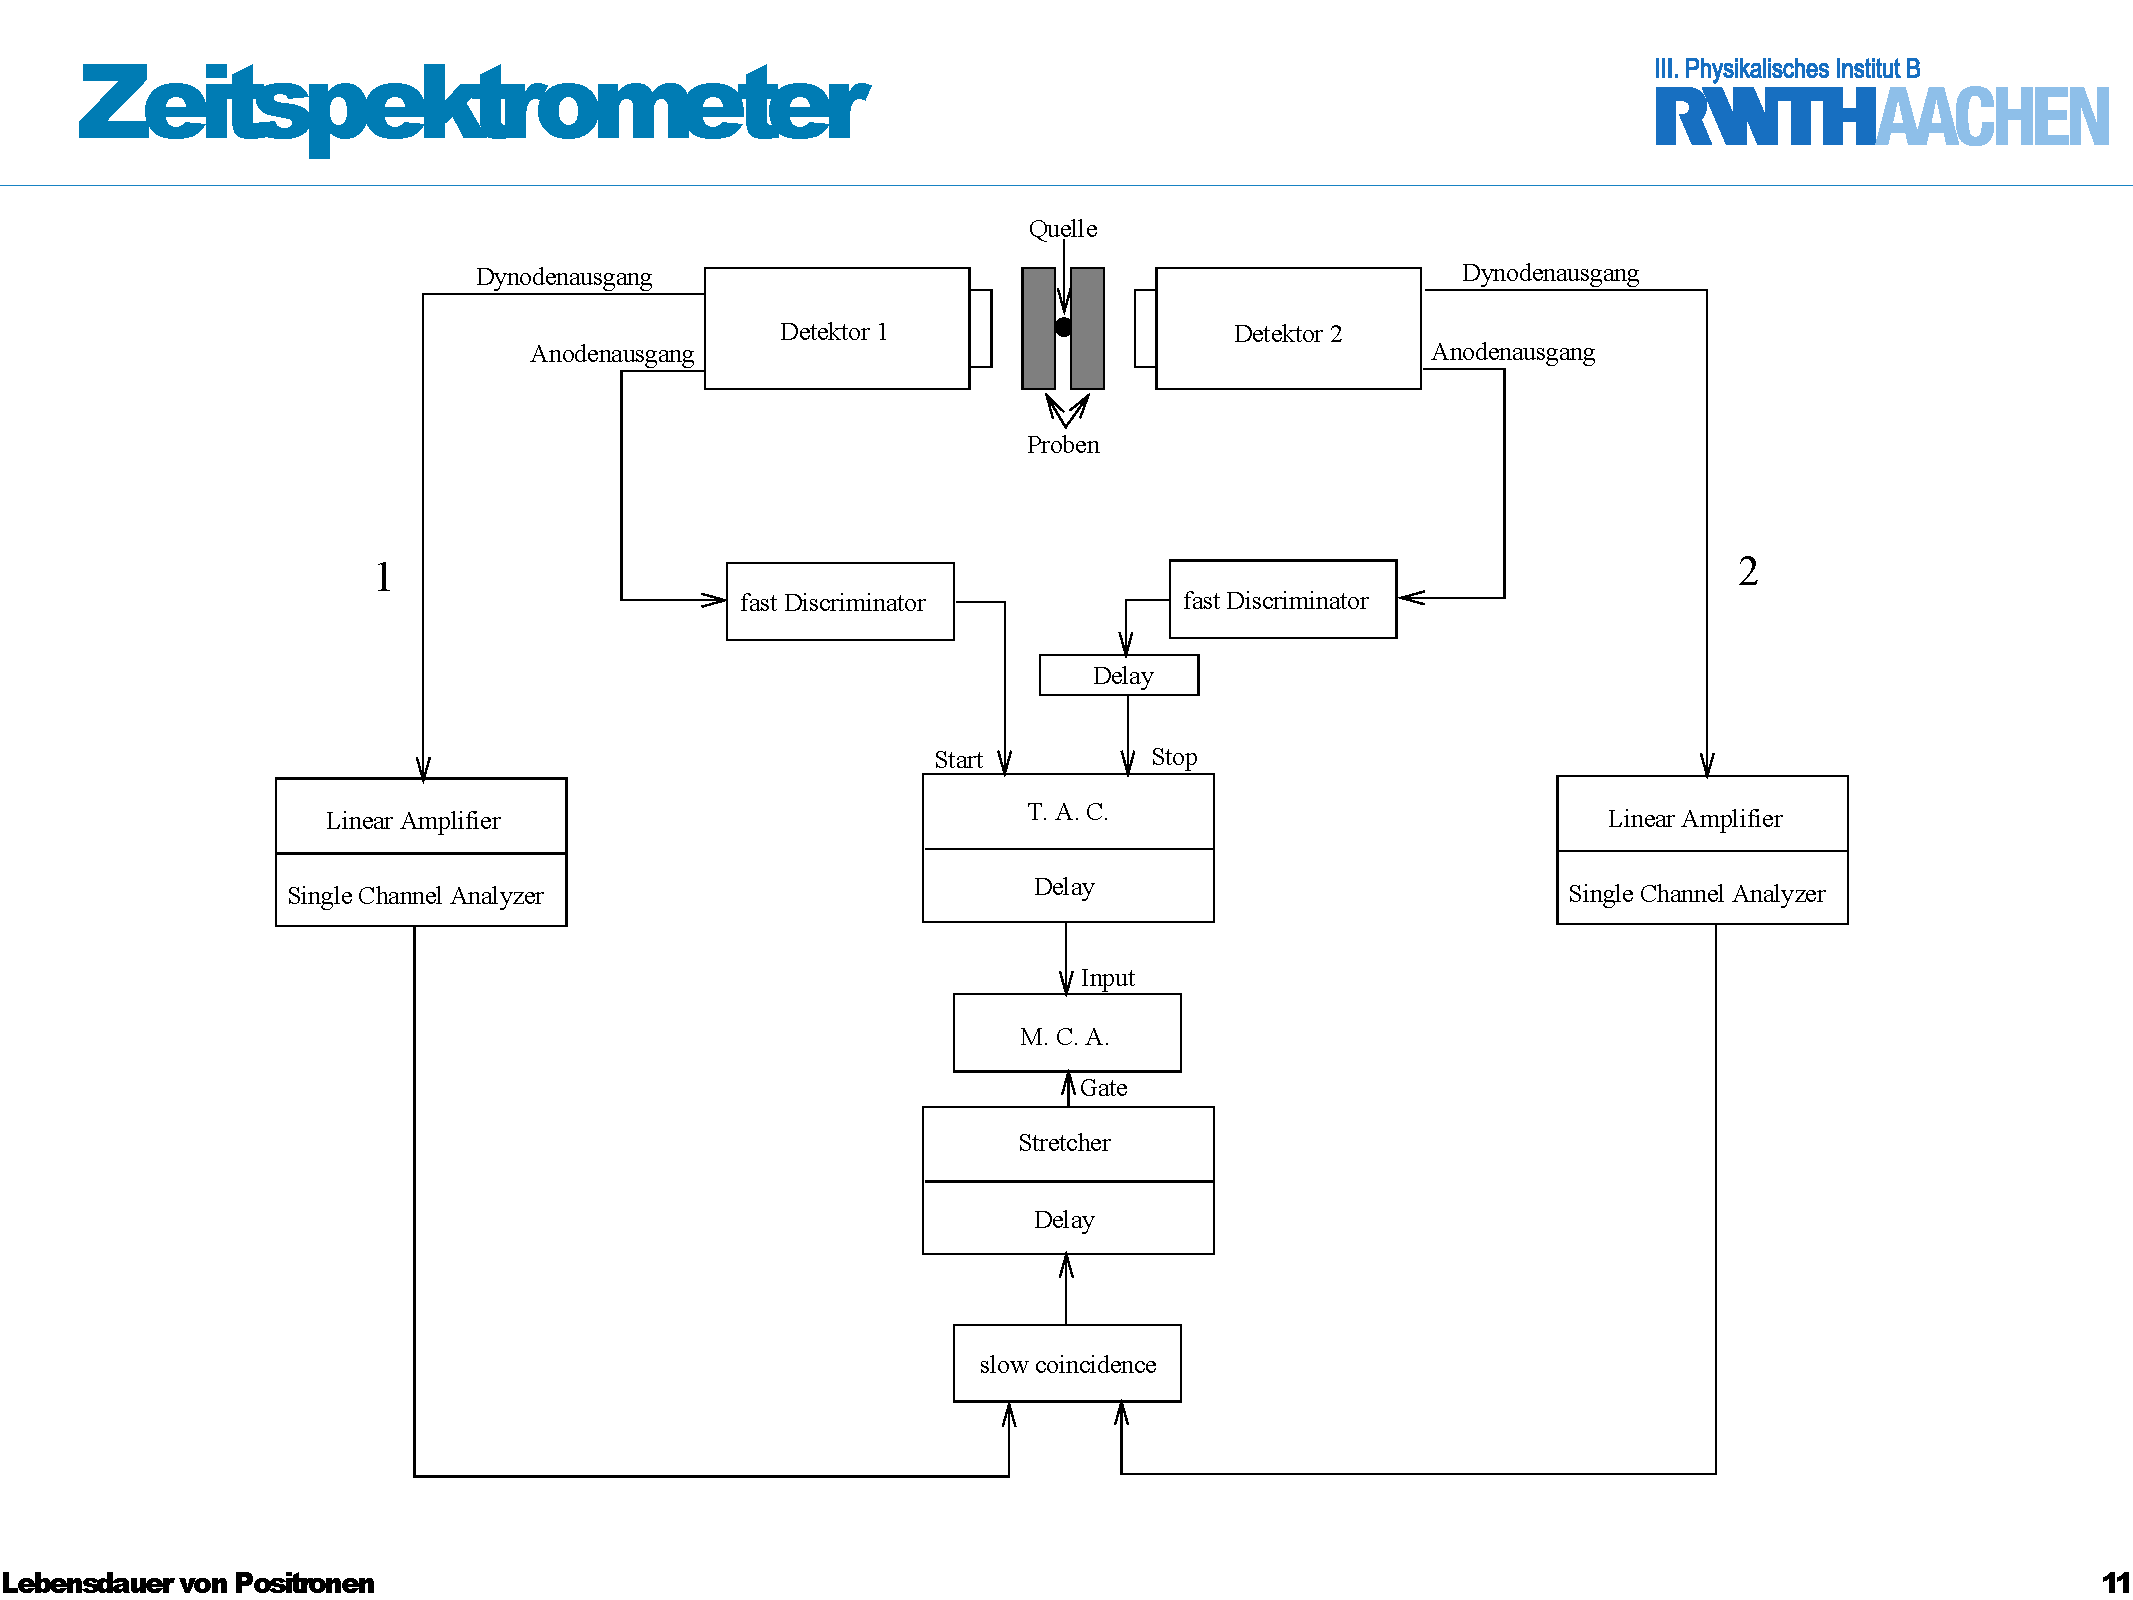
\includegraphics[width=0.8\textwidth]{schaltplan.pdf}
		\caption{Schaltplan}
		\label{fig:schaltplan}
\end{figure}
Der Detektor besteht aus zwei zylindrischen Szintiallatonsdetektoren,
 welche in einem Gehäuse mit einem Photomultiplier verbaut sind. Die radioaktiven Proben werden zwischen beiden Szintillatoren
platziert. Die Photomultiplier werden mit einer Spannung von $2\si{kV}$ betrieben. Von beiden Photomultipliern
wird sowohl das Anodensignal als auch das Dynodensignal abgegriffen und für das Messen und Triggern der 
Zeitabstandsmessung genutzt. Hierbei liefert jeweils ein Photomultiplier das Start und der andere 
das Stoppsignal für die Zeitmessung liefert.
Die elektronische Signalverabreitung unterteilt sich in zwei Schaltkreise
 (siehe Abbildung \ref{fig:Schaltplan} für eine Blockdarstellung des gesmaten Schaltplan): \\
\begin{itemize}
	\item
	Ein "langsamer Kreis" dieser prüft ob die gemessenen Photonen sich im richtigen Energieintervall 
	befinden und erzeugt abhängig davon ein Triggersignal.
	\item Ein "schneller Kreis" dieser bestimmt die Zeitdifferenz und gibt dieses in Form eines Pulses an einen
	Vielkananlanalysator weiter, sofern ein Triggersignal vom "langsamen Kreis" besteht.	
\end{itemize}
\subsection*{langsamer Kreis}
	Für den langsamen Kreis wird das Dynodensiganl der Photomultiplier genutzt und in jeweils einem 
	Einzelkanaldiskriminator (\mathbf{SCA}) weiter verarbeitet, dieser verstärkt das Signal zunächst (es wird
	ein Gain von 300 eingestellt). 
	% Erklären was beim Differenzieren passiert.
	Das Dynodensignal beitzt eine ausreichende linearität zwischen Energie und Pulshöhe und es ist möglich
	zunächst ein Energiespektrum mit Hilfe des Vielkanalanalysator aufzuzeichnen.
	Anschliessend werden die Schwellwerte im Einzeldiskriminator so eingestellt, dass nur Teilchen mit einer höheren
	Energie als der rechten Flanke des Anhilationspeak als Startsignal (Fenster 2) genutzt wird und Teilchen
	mit einer niedrigeren Energie als Stoppsignal. Zusätzlich wird für das Stoppsignal eine untere Grenze bei ???
	eingestellt um den Untergrund durch niederenergetischer Teilchen und elektronisches Rauschen des Photomultiplier
	zu reduzieren. Nachdem die Fenster für Start und Stoppsignal zunächst mit dem verstärkten Dynodensignal eingestellt sind,
	wird nun ein Ausgang der Einzelkanaldiskriminatoren genutzt, der logisches Ausgangssignal liefert.
	Über eine integrierte Koinzidenzschaltung der SCA verbunden. Wenn nun Signale von beiden SCA innerhalb des Koinzidenzzeitfenster
	gemessen werden, wird ein logisches Signal an einen Gategenerator weiergeleitet. Der Gategenenerator liefert ein Ausgangssignal, dass
	am Vielkanalanlysator das Gate zur Datennahme öffnet.
	 
		\includegraphics[width=0.8\textwidth]{../analyse/auswahl.pdf}
		\caption{Energiespektrum von $^{22}$Na. Gemessen aus dem Dynodensignal und vorverstärkt,geglättet im Einzelkanaldiskrimnator}
		\label{fig:schaltplan}
\end{figure}

\subsection*{langsamer Kreis}
	Für den langsamen Kreis wird das Dynodensiganl der Photomultiplier genutzt und jeweils in einem 
	Einzelkanaldiskriminator (\textbf{SCA}) weiter verarbeitet, dieser verstärkt das Signal zunächst (es wird
	ein Gain von 300 eingestellt). 
	% Erklären was beim Differenzieren passiert.
	Das Dynodensignal beitzt eine ausreichende linearität zwischen Energie und Pulshöhe und es ist möglich
	zunächst ein Energiespektrum mit Hilfe des Vielkanalanalysator aufzuzeichnen.
	Anschliessend werden die Schwellwerte im Einzeldiskriminator so eingestellt, dass nur Teilchen mit einer höheren
	Energie als der rechten Flanke des Anhilationspeak als Startsignal (Fenster 2) genutzt wird und Teilchen
	mit einer niedrigeren Energie als Stoppsignal (Fenster 2). Zusätzlich wird für das Stoppsignal eine untere Grenze bei ???
	eingestellt um den Untergrund durch niederenergetischer Teilchen und elektronisches Rauschen des Photomultiplier
	zu reduzieren. Nachdem die Fenster für Start und Stoppsignal mit dem verstärkten Dynodensignal eingestellt sind,
	wird nun ein Ausgang der Einzelkanaldiskriminatoren genutzt, der logisches Ausgangssignal liefert. Das Signal wird 
	über eine integrierte Koinzidenzschaltung der SCA verbunden. Wenn nun Signale von beiden SCA innerhalb des Koinzidenzzeitfenster
	gemessen werden, wird ein logisches Signal an einen Gategenerator weitergeleitet. Der Gategenenerator liefert ein Ausgangssignal, dass
	am Vielkanalanlysator das Gate zur Datennahme öffnet.
\subsection*{schneller Kreis}
	Für den schnellen Kreis wird das Anodensigal der Photomultiplier genutzt. Start und Stoppsignal werden zunächst in jeweils einem Constant
	Fraction Discriminator (\mathbf{CFD}) weiter verarbeitet, dieser erzeugt durch differenzieren zunächst einen bipolaren Puls aus dessen Nulldurchgang
	ein von der Pulsform unabhängiges Zeitsignal erzeugt wird und in Form eines logischen Signal ausgegeben wird. Die Signale von beiden
	CFD werden von einem Time Analyzer verarbeitet. Der Time Analyzer erzeugt einen Puls, abhängig vom Zeitlichen Abstand von Start und Stoppsignal,
	der im VKA aufgenommen und in ein Pulshöhenspektrum umgesetzt wird. Um den schnellen und langsamen Kreis zeitlich aufeinander 
	anzupassen ist zusätzlich eine Verzögerungseinheit zwischen Time Analyzer und VKA geschaltet.
\section{Ergebnisse}

\section{Diskussion}
\end{document}
